\chapter{Introduction}
\label{chap:introduction}

The global flow of Foreign Direct Investment (FDI) has risen from almost nothing
in the 1970s to over \$2.3 trillion dollars in 2016, becoming an important
source of global capital (Figure~\ref{fig:globalfdi}). For developing countries
especially, capital from multinational corporations (MNCs) is robust to global
economic downturns, prompting major international organizations to endorse FDI
as a key factor to economic development and poverty reduction
\citep{Mallampally1999, WorldEconomicForum2013}.\footnote{Indeed, while FDI into
  developed economies dropped almost 50\% during the 2000 recession and the 2008
  financial crisis, FDI into developing countries only experienced a plateau or
  a small reduction. More recently, as global FDI flow slipped in 2016 and 2017,
  FDI into developing countries still remained stable \citep{UNCTAD2018}.} Within the scholarly
field of International Political Economy (IPE), much of the literature starts
with the view that countries will always seek FDI for its various benefits
\citep{Jensen2008b}. Works in IPE tend to focus on \textit{how} countries can
attract FDI, and do not question \textit{whether} they want to do so
\citep{Jensen2003, Li2003, Li2006, Ahlquist2006}.\footnote{Two recent exceptions
  are \citet{Pinto2013, Pandya2016}, who are the first to examine variation in
  countries' demand for FDI.}

\begin{figure}[tbp]
  \centering
  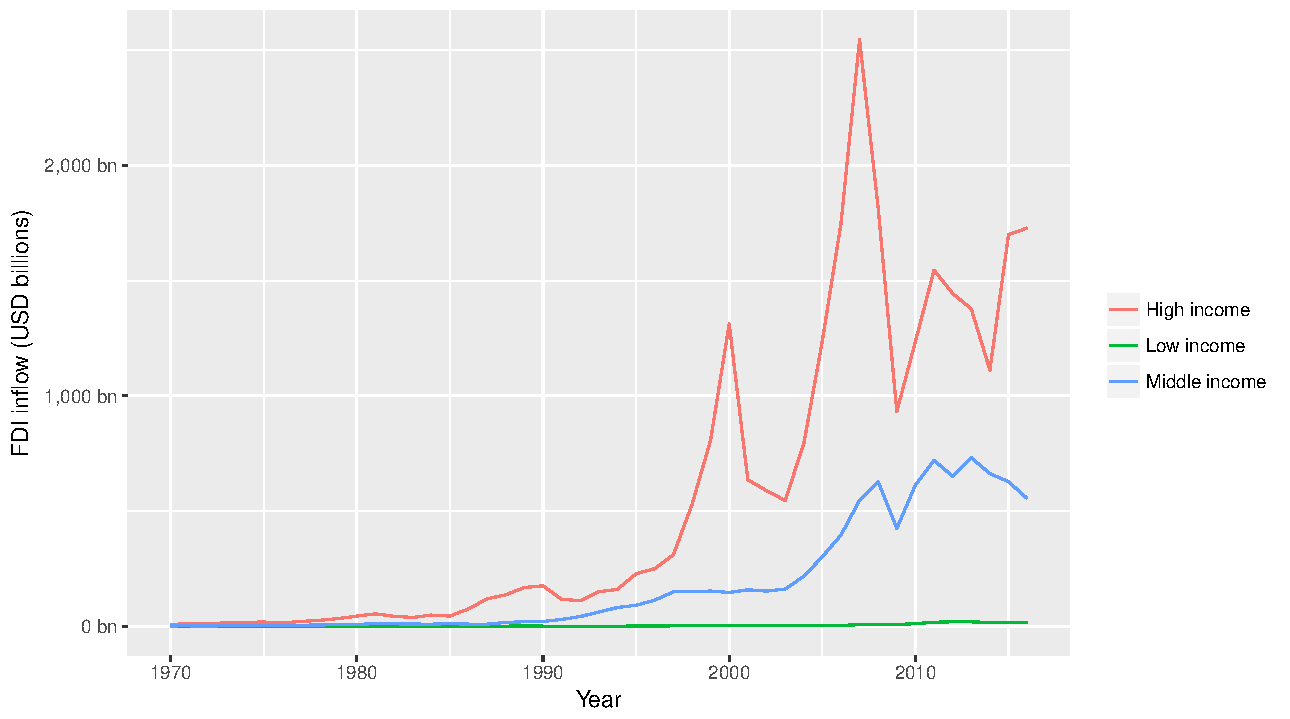
\includegraphics[width=0.8\textwidth,keepaspectratio]{../figure/global_fdi}
  \caption[FDI global inflow, 1970-2006.]{FDI global inflow, 1970-2006. The last
    four decades witness the growth of FDI into the most important source of
    global capital. Source: World Bank's World Development Indicators.}
  \label{fig:globalfdi}
\end{figure}

At first glance, the benefits of FDI seem obvious. FDI brings capital, create
jobs, contribute tax revenue, and promise technological spillover to the local
economy. Consider the impact of a high-tech facility by Intel on Vietnam's
economy. In 2006, Intel announced Saigon Hi-tech Park in Ho Chi Minh City,
Vietnam as the site for its largest chip testing and assembly in the world.
Starting from the initial plan of a US\$300 million facility, Intel decided
eight months later to increase the investment to US\$1 billion dollar, making up
almost 10\% of Vietnam's registered FDI in 2006. In 2016, Intel Products Vietnam
(IPV) employed 4000 workers at full capacity, exported US\$3.45 billion worth of
goods (18.2\% of Vietnam's electronics export), and contributes more than
US\$100 million to Vietnam's GDP in tax payment, salary, and profit. More
importantly, IPV also helped Vietnam address the skill shortage in engineering
and management. In the beginning, IPV hired workers earlier and trained them at
other Intel facilities in Asia. In the longer term, IPV developed an engineering
education program in partnership with Arizona State University and local
universities, training thousands of young Vietnamese engineers and giving them a
job. As a result, IPV's workers are vastly more productive: while IPV's
workforce only constituted 5\% of all workers at the Saigon Hi-tech Park, its
export value amounted to 72\%. Finally, Intel's decision to choose Ho Chi Minh
City over other candidate sites, including Chennai (India), Bangkok (Thailand),
and Dalian (China), was a significant marketing boost to Vietnam's image as a
destination capable of high-tech manufacturing. Following Intel, many other MNCs
opened high-tech facilities in Vietnam, including Samsung's three factories (in
2009, 2013, and 2014), Nokia/Microsoft (2012), and LG (2013) \citep{Dinh2016,
  UNCTAD2008}.

From a theoretical perspective, \citet{Findlay1978} argues that FDI plays a key
role in economic growth by upgrading the local economy's technological capability. As
well-known from neoclassical growth theory, diminishing returns to capital will
at one point stop capital from accumulating further, preventing long-run
economic growth from being driven by capital accumulation alone
\citep{Solow1956}. FDI can counteract this dynamic by helping local workers and
suppliers upgrade their productivity, either via training or demonstration.
In other words, technological spillover from FDI shifts the domestic factor-price
frontier to the right, resulting in a continually increasing capital stock and
sustained economic growth.

However, despite the theoretical arguments and shining examples such as Intel in
Vietnam, cross-country studies shows that
not all FDI are the same and that its effects are highly conditional. For
example, there is no conclusive evidence of FDI inflow having a positive effect on
growth \citep{Nair-Reichert2001, Carkovic2002} or poverty reduction
\citep{Guerra2009}. This puzzle opens a substantial literature on how the
growth-enhancing and spillover effect of FDI is conditional on the absorptive
capacity of the host economies, i.e. its level of human capital, technological
sophistication, and financial market development \citep{Durham2004,
  Nunnenkamp2004, Fu2008, Willem2004}. In addition, while the capital brought
and jobs created by FDI may be unconditionally good for the overall economy, its
distributional effects cut across constituencies in the host economy, creating
political cleavage across both sectoral and geographical divides
\citep{Chintrakarn2012, Goldberg2007, Nunnenkamp2007}.

Given the evidence on the conditional effect of FDI, it is no longer tenable to
assume that countries' preference for FDI is homogeneous. By holding this
assumption, we neglect the role of the state in shaping global capital flow,
falling prey to the discredited ``race to the bottom'' thesis of globalization
\citep{Mosley2005}. Arguably, examining countries' preference for FDI should be
of more interest to political scientists than the current focus on determinants
of MNCs' location, which often amounts to adding a political variable to an
existing economic model of FDI flow. In addition, even if we only care about
MNCs' preference, to get an accurate estimate we must still take into account
countries' preference. For example, consider the received wisdom that
democracies receive more FDI \citep{Jensen2008a}. Without controlling for
countries' preferences, it is difficult to interpret this finding as democracies
actively pursuing MNCs or as MNCs finding democracies attractive.

\section{Goal of the research}

My research aims to estimate the preference of countries and MNCs for each
other. I develop an empirical strategy that takes into account the two-sided
nature of the FDI market, i.e. a subsidiary can only materialize if both the MNC
and the host government agree. Recognizing that this two-sided matching dynamics
can also be found in the labor or the marriage markets, I adapt the statistical
models first developed in Sociology for labor and marriage markets and apply
them to the study of FDI \citep{Logan1996, Logan2008}.

In doing so, I simultaneously address three long-standing issues in the FDI
literature. First, I ``bring the state back in,'' filling the gap in the literature on the
variation of countries' preference for FDI.\footnote{\citet{Evans1985}'s
book argues that states are weighty actors with their own capabilities and
initiatives rather than an arena for societal and interest groups to negotiate
for their share. Here, I argue that states are weighty actors with their own
preferences rather than goods that MNCs pick and choose.} Two notable exceptions are
\citet{Pinto2013} and \citet{Pandya2016}, whose pioneering works propose
partisan politics and regime types as factors shaping preferences for FDI.
However, while their theories are ground-breaking, the empirical estimation of
countries' preference remains inadequate. In addition, these researchers have
not used their findings to re-estimate the preference of MNCs and disentangle
the ``push'' and ``pull'' factors of FDI flow.\footnote{``Push factors'' refer
  to characteristics of the home country and of the MNC, pushing capital out
  from its origin. ``Pull factors'' refer to the characteristics of the host
  country, pulling capital towards its destination.} Using a two-sided matching
model, I will naturally be able to estimate both sides' preference.

Second, I propose that we need to pay more attention to countries' preference
for different types of FDI. While the IPE literature has largely focused on the
quantity of FDI flow, countries pay much attention to the its type, using
various incentives and restrictions to target certain types of FDI. Indeed, MNCs
come with varying amount of capital, labor demand, and technological
sophistication, all of which have different effects on the host country's
economy. Just as the two-sided matching model can estimate MNCs' utility
function for countries' characteristics (e.g. market size, level of
development), it can also estimate countries' utility function for MNCs'
characteristics (e.g. technological sophistication, export strategy).

Third, while the majority of the literature uses FDI flow data, these data
are accounting constructs created to keep track of countries' balance of payment
and thus map poorly to concepts in Political Science theories. Very often, the
variable of interest in our theories is the scale of MNCs' activities in the
host country, which can be very different from the amount of border-crossing
capital thanks to MNCs' complex financial and tax strategies \citep{Kerner2014}.
Therefore, we would do much better testing our theories with firm-level
operational data. Because the two-sided matching model is a behavioral model in
which each actor's decision is a unit of observation, and we can naturally use
it to analyze firm-level data.

These three issues are related and represent the status quo in the FDI
literature. Data limitation forces scholars to look at country-level aggregate
FDI flow, making it difficult to study countries' preference for FDI types. And
without studying countries' preference, our current models of MNCs' location
choice are also suspect.

In sum, my dissertation benefits the field by using firm-level data to estimate
both firms' and countries' preference for each other's characteristics. In this
two-sided matching model, MNCs and countries evaluate their available options
according to their utility functions, choose the best alternative, culminating
in an MNC's subsidiary located in a host country.

Estimating this model would be straightforward if we observed not only
subsidiaries' locations but also their set of options (called their
``opportunity set'' in the matching literature).\footnote{Discrete choice models
  can be used to estimate the utility function when both the choice and the set
  of options are observed. Indeed, discrete choice models remain the dominant
  empirical approach in the industrial location literature, effectively ignoring
  the fact that not all MNCs have the same set of location options
  \citep{Arauzo-Carod2010}.} Unfortunately, while data on subsidiaries' location
are available, the opportunity set is generally unobserved as researchers cannot
peek into the negotiation process between countries and MNCs. The two-sided
matching model solves this problem by using the Metropolis-Hastings (MH)
algorithm, a Markov chain Monte Carlo (MCMC) approach that repeatedly samples
new opportunity sets and rejects them at an appropriate rate to approximate
their true distribution. In addition, the estimated preference parameters in the
two-sided model have a convenient interpretation as the relative weight of
different variables on MNCs' and countries' utility. This allows us to make
statements such as: ``In evaluating MNCs, China values a 2\% increase in the
firm's capital as much as a 1\% increase in labor demand.''

\section{Roadmap}

In the rest of this introductory chapter, I review in-depth the three issues in
the literature of FDI's political determinants, outlining the current attempts
to address them and how my approach can contribute to the solution.

In Chapter~\ref{chap:model}, I describe the two-sided matching model, including
both its game-theoretic origin and its statistical estimation.
Chapter~\ref{chap:simulation} uses simulations to demonstrate the correctness of
the model and explore its characteristics. Chapter~\ref{chap:labor} applies the
model on US labor market data, the original domain of the two-sided matching
approach, in order to compare with and expand upon previous results.
Chapter~\ref{chap:FDI} brings us back to the study of FDI, applying the model on
firm-level data of Japanese MNCs in East and Southeast Asia.
Chapter~\ref{chap:conclusion} concludes and explores potential applications of
the two-sided matching model in other areas of Political Science.

\section{Three issues in the FDI literature}
\label{sec:literature_issues}

\subsection{Estimating countries' demand for FDI}

The IPE literature on the political determinants of FDI has overwhelmingly
focused on what MNCs demand from countries, not what countries demand from MNCs.
In this literature, politics matters, but only in terms of what
political factors make countries attractive to MNCs. As Jensen states in
the introduction of \textit{Nation-states and the multinational corporation}:

\begin{quote}
  Which government policies prove beneficial to multinational corporations?
Which political institutions provide multinational corporations with credible
commitments to these market-friendly policies? These emerge as the central
questions of this book.
\end{quote}

Other scholars share the same line of inquiry \citep{Ahlquist2006, Busse2007,
  Buthe2008, Li2003}. In their theoretical argument, the central dynamics of the
negotiation between countries and MNCs is that FDI is mobile before MNCs make
the investment on the ground but immobile after. Since the cost of relocation is
higher the more investment MNCs commit, the original bargain between the host
country and the MNC become increasingly obsolete as the host country can alter
the original bargain at the expense of the MNC, knowing that relocating would
cost the MNC dearly. Therefore, certain political
institutions, such as democracy, veto players, and federalism, increase FDI
inflow because they can credibly commit not to change their policies \textit{ex
  post}, and are thus
attractive to MNCs.

Cost of doing business arguments. 

In theorizing FDI inflow largely as a function of MNCs' preference, the FDI
literature implicitly assumes that countries are eager to receive as much FDI as
possible. The two common empirical approaches in the literature expose this
assumption. In the first approach, researchers build a regression model with FDI
inflow as the dependent variable and a political factor as the independent
variable of interest. The problem with this model is that it is impossible to
interpret the political factor as an attraction to MNC or as a motivator of
countries' demand for FDI. Consider \citet{Jensen2005}'s finding that federalism
is positively associated with FDI inflow. The authors interpret this correlation
as federalism constraining the whim of the central government, increasing policy
stabilities, and thus making the country attractive to MNCs. However, the
alternative explanation is that local governments in a decentralized system
compete more intensely for FDI, driving up the FDI inflow. For example, As China
decentralized in the late 1980s and early 1990s, local governments gained the
authority to approve foreign investment up to a certain size, thus able to court
MNCs without asking the central government for permission.\footnote{Similar to
  China's broader economic reform, decentralization in China's FDI policies
  happened incrementally. In 1979, China first allowed FDI in four Special
  Economic Zones, i.e. Shenzhen, Zhuhai, Shantou (near Hong Kong), and Xiamen
  (near Taiwan). As the economic benefits of FDI became clear, provinces started
  clamoring for the ability to attract FDI themselves. Therefore, in 1984, China
  allowed 14 coastal cities to approve FDI projects themselves, and in the early
  1990s, allowed inland regions to do the same. \citet{Gallagher2002, Shirk1993}
  discuss how the coalition for decentralization expanded over this period, and
  \citet{Coase2012} provides a historical account of China's economic reform
  more broadly.} In addition, local governments could keep all revenue in excess
of a quota pre-negotiated with the central government, further motivating them
to bring in MNCs as a lucrative source of tax revenue. Having both the authority
and the incentive to attract MNCs, Chinese local governments engaged in an
intense competition for MNCs. For example, while there were only 117 development
zones in 1991, the number exploded to 2700 in 1992, of which only 95 were
initiated by central ministries \citep{Montinola1995}. Far from
\citet{Jensen2005}'s argument, China's federalism did not increase FDI inflow by
producing a static policy environment that MNCs like. On the contrary,
federalism incentivized Chinese local governments to demand FDI, fostering
local policy experiments that were anything but stable.\footnote{A very similar
  account of decentralization causing provincial demand and competition for FDI happened in Vietnam
  as well \citep{Malesky2004c}.}

In the second approach, researchers estimate MNCs' preference using discrete
choice model. The dependent variable is the MNC's choice of a location over all
the others, and the independent variable of interest is a characteristic of the
location \citep{Arauzo-Carod2010}. In discrete choice model, the assumption is
that all locations are available for the MNC to pick and choose, effectively
ruling out the possibility that the host country can decline the MNC's
investment proposal. Such an assumption is unfounded. For example, in 2007, Da Nang, a
central province of Vietnam known for its public governance quality, turned down
\$2.5 billion dollars from
a Taiwanese-Japanese steel factory and a Japanese paper pulp factory for
environmental concern \citep{NLD}. In 2014, even in tough times, when Da Nang's and Vietnam's
FDI inflow was
merely half of the previous year, Da Nang's attitude towards FDI remained
selective, declining a \$200-million Hong Kong textile factory and a 30-hectare Korean dying
facility, showing its  

A historical and comparative examination of FDI policies makes it clear that the
assumption of countries' unequivocal demand for FDI is not true. First,
historically countries are not so open to FDI.

Second, there is substantial variation across countries.

Third, countries are very strategic in their FDI policies, changing it over
time to fit with the political and economic conditions of the countries.


We have made this mistake before. Despite earlier pessimism about countries engaging in a race to the bottom to
attract footloose global capital, empirical evidence shows that countries'
policies still vary substantially \citep{Drezner2001}. While the broader IPE
literature has recognized the variation in countries' trade, welfare,
environmental, and fiscal policies in the face of globalization, we have
surprisingly done less work to explain variation in countries' demand for FDI.
Neglecting countries' demand for FDI is both a theoretical and an empirical gap
in our FDI literature. Theoretically, much of the literature on the political
determinants of FDI only examines how the political factors are assessed by the MNC, assume that countries want as much FDI as possible and the
only problem is that they cannot credibly commit to reduce the uncertainty in
order to attract business. On the empirical side, in using discrete choice model
to model MNCs' location decision, the literature assumes that all MNCs have
access to all locations.

Recognizing this gap in the literature, \citet{Pinto2013} and \citet{Pandya2016}
recently broke ground in this area. Similar to the rich IPE literature in
international trade, these studies argue that countries' demand for FDI varies
according to FDI's distributive effect on their domestic constituencies
\citep{Broz2001, Milner2005a}. In this theoretical framework, labor supports FDI
because foreign firms bring capital that increases the demand for labor and
raises productivity, both of which lead to higher wage. On the other hand,
domestic firms oppose FDI because foreign firms compete for local labor, inputs,
and markets. Both \citet{Pinto2013} and \citet{Pandya2016} formulate their
theories as a variant of this labor-vs-business tension, which surfaces in the
former work as left-vs-right governments, and in the latter as
democratic-vs-authoritarian regimes.

While these pioneering works have enriched our understanding of the relationship
between politics and FDI, their empirical approaches do not satisfactorily
measure countries' demand for FDI, leaving their theoretical arguments untested.

Consider \citet{Pinto2013}'s approach. The author controls for economic and
institutional factors that affect FDI flow into a country, then claims that
what's left in the residual is the country's demand for
FDI.\footnote{Specifically, the estimation of FDI openness involves two steps.
  First, the author runs a gravity model explaining bilateral FDI flows,
  estimating the intercept as the host country-year fixed effect. Second, this
  fixed effect is then regressed on several economic and endowment factors of
  that country-year (i.e. GDP, GDP per capita, average school years, arable
  land). The residual in the second stage is considered the country's ``FDI
  openness'' in that year.} For this approach to be valid, every economic,
institutional, and endowment factors that affect FDI flow has to be controlled
for, leaving only the country's demand in the error term. This claim is much
stronger than the common assumption of exogenous error, which is valid as long
as the omitted factors are uncorrelated with the independent variable of
interest. Framed substantively, since the residual is likely to contain more
than just the country's demand for FDI, if we observe an abnormally high level
of FDI, we do not know whether it is because the country welcomes FDI or because
MNCs find something attractive in the country.\footnote{In addition, this
  approach requires data on bilateral FDI flow, ideally disaggregated by
  sectors. Therefore, this approach is limited to OECD countries only
  \citep{Pinto2008}. During the period the authors study, 1980-2000, OECD
  countries account for 95\% of global FDI outflow and 90\% of inflow. However,
  since then the role of the developed world in global FDI has declined sharply,
  reducing to 60.8\% of outflow and 40.6\% of inflow in 2014
  \citep{UNCTAD2015}.}

In contrast to \citet{Pinto2013}'s statistical approach, \citet{Pandya2014,
  Pandya2016} attempts to find a proxy for countries' demand for FDI. The author
uses the annual US Investment Climate Reports to construct the number of
industries that have foreign ownership restrictions or face investment
screening. The advantages of this measurement are its ease of interpretation and
its availability for many countries. However, two problems remain. First, adding
up the raw count of restricted industries is not appropriate because industries
are not the same. For example, given the reach of the banking sector into all
corners of the economy, a country's opening up its financial industry indicates
much more FDI-friendliness than, say, allowing foreign furniture makers to set
up shops. Since the theoretical argument is driven by FDI's distributive effect,
we must not ignore the varying impact of FDI across sectoral constituencies.

Second, according to the coding rule, an industry is coded as free if there is
no mention of restriction. However, when there is little FDI, US Investment
Climate Report may find it not worth mentioning and does not report the
restrictions. Therefore, ``zero restriction'' in the dataset can either mean
that a country is very closed or very open to FDI. This concern is not
hypothetical. Figure \ref{fig:china_fdi_restriction} shows that, following the
coding of the US Investment Climate Reports, China seemed 100\% open to FDI up
until 1986 when it started imposing restrictions. The reality is the opposite.
Prior to 1986, only limited FDI was allowed as joint-venture in Special Economic
Zones (SEZ). The year of 1986 was, in fact, the first time China allowed any
wholly owned FDI outside of SEZs.

\begin{figure}[tbp] \centering
  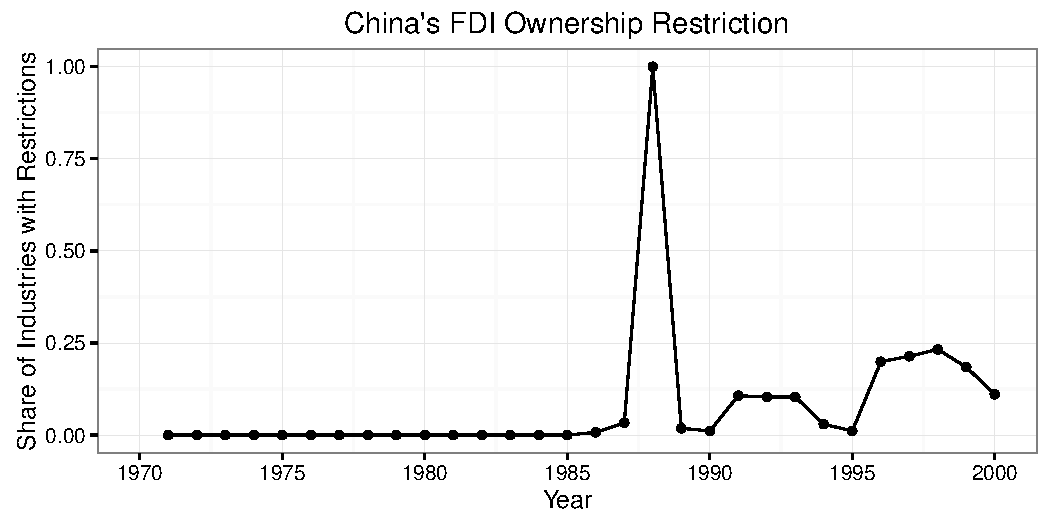
\includegraphics[width=0.8\textwidth,keepaspectratio]{china_fdi_restriction}
  \caption[China's FDI ownership restriction.]{China's FDI ownership
    restriction, as coded in \citet{Pandya2010}. Prior to 1986, FDI in China was
    limited to few experimental Special Economic Zones, and thus not mentioned
    in US Investment Reports. The sharp spike in 1988 also does not seem to
    correspond to any actual change in policy, and likely another artifact of
    reporting. (See \citet{Zebregs2002} for a historical overview of China's FDI
    policy.)}
  \label{fig:china_fdi_restriction}
\end{figure}

The two-sided matching model circumvents these thorny measurement issues by
modeling countries' demand for FDI directly. Intuitively, if we observe that a
country welcomes certain firms to invest but not others, we can compare the
characteristics of the invited and the uninvited firms to infer that country's
preference for FDI.

\subsection{Estimating countries' preference for types of FDI}

In addition to estimating countries' demand for FDI, we should also examine
countries' preference for different types of FDI. Indeed, while the Political
Science literature has focused almost exclusively on the quantity of FDI,
treating all FDI as one homogeneous flow of capital, policy makers seem to pay
much more attention to distinguishing its types. Commenting on the role of
International Investment Agreements, \citet{UNCTAD2015} says, ``Today,
increasing the quantity of investment is not enough. What matters is its
quality, i.e. the extent to which investment delivers concrete sustainable
development benefits.'' Governments in developing countries all offer various
forms of tax incentives and fee waivers to attract FDI that invests in a remote
region, brings new technology, or focuses on exporting \citep{Ricupero2000}. For
example, since 2006, China's official FDI policy has been ``quality over
quantity,'' promoting FDI with intense R\&D in high-productivity sectors
\citep{Guangzhou2011}.

Despite the importance of disaggregating FDI by its type, two data limitations
prevent researchers from doing so. First, FDI flow data typically does not
disaggregate into types of FDI. \citet{Alfaro2007} attempt to get around this
problem by using Germany's sectoral skill intensity as the proxy for the FDI
quality from each sector in the OECD. To do so is to assume that 1) Germany's
sectoral variation is the same as everyone else's in the OECD, and 2) there is
little variation in skill intensity within a sector. Both assumptions are
untenable, especially since the authors divide all manufacturing industries into
only two categories: low skill and high skill.

Second, even if we can differentiate types of FDI, it remains an open question
how to estimate countries' preference for them. \citet{Alfaro2007} use
information from IPAs' website and survey response as a proxy for their
countries' preference---if an IPA lists an industry as a ``target industry,''
the authors say that the country wants to attract that type of FDI. While this
approach seems reasonable at first glance,
Figure~\ref{fig:IPA_target_industries} shows that there is little variation in
what IPAs claim to be their target industries. Because investment promotion is
mainly a marketing and aspirational exercise, almost everyone claims that they
target manufacturing, advanced manufacturing, and infrastructure. In addition,
if we use IPAs as a proxy for countries' preferences, we should also model the
selection process in which the countries that decide to establish an IPA may not
be the same as those who do not. Both of these issues are not addressed by
\citet{Alfaro2007}, and we are still in need of a way to estimate countries'
preference for different types of FDI.

\begin{figure}[tbp] \centering
  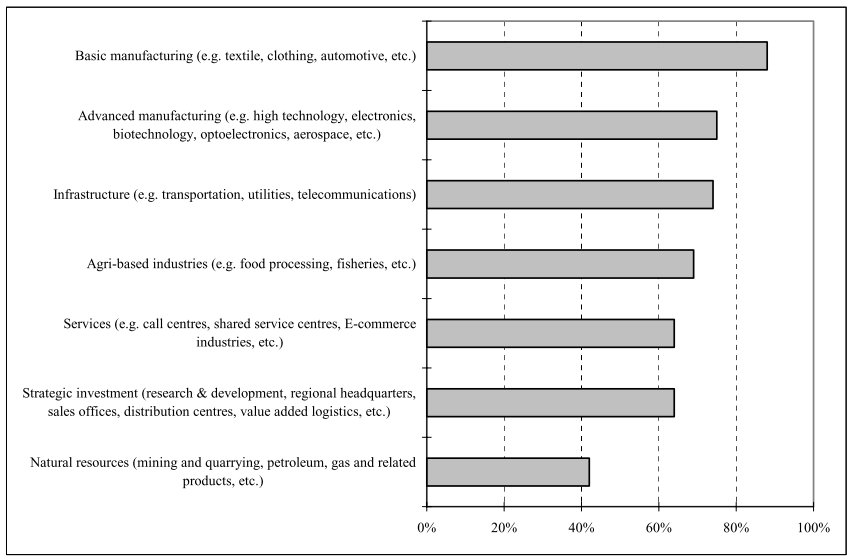
\includegraphics[width=\textwidth,keepaspectratio]{../figure/IPA_target_industries}
  \caption[Target industries by IPA around the world.]{Target industries by IPAs
    around the world. Because of the image building aspect of investment
    promotion, almost all IPAs say that they want to attract ``manufacturing,''
    ``advanced manufacturing,'' and ``infrastructure.'' Therefore, using what is
    listed as investment priorities may not be a reliable way to measure
    countries' preference for FDI. Source: \citet{UNCTAD2001}}
  \label{fig:IPA_target_industries}
\end{figure}

In sum, differentiating FDI by sectors only gives us a crude typology of FDI. We
can address this challenge using firm-level data, giving us information on not
only a firm's sector but also its operational characteristics, such as research
and development (R\&D) expenditure or export intensity. These measures are
firm-specific and get closer to what countries are looking for in FDI projects.
Using R\&D expenditure or export intensity as firms' characteristics in the
two-sided matching model, I will be able to estimate countries' preferences for
these traits.

\subsection{Measuring MNCs' activities}

As \citet{Kerner2014} argues, the IPE literature on FDI is a bit of a misnomer.
Political scientists are rarely interested in FDI \textit{per se}---rather, they
are interested in the activities of MNCs, which in turn, affect other important
issues such as nation-state autonomy \citep{Mosley2005}, economic development
\citep{Moran1998}, labor standards \citep{Mosley2007}, and environmental
policies \citep{Prakash2007}. However, while the theory involves MNCs as the
central actor in the causal mechanism, the empirics often uses FDI flow as the
variable of interest. These two concepts---the level of MNCs' affiliate
activities in a country and FDI inflow into a country---are not the same.

Consider the definition of FDI from UNCTAD, the main producer of FDI data widely
used by researchers:

\begin{quote} FDI has three components: equity capital, reinvested earnings and
  intra-company loans.
  \begin{itemize}
  \item Equity capital, i.e. the foreign investor’s purchase of shares of an
    enterprise [in the host country].
  \item Reinvested earnings, i.e. the foreign investor’s share \ldots of
    earnings not distributed as dividends by affiliates, or earnings not
    remitted to the foreign investor.
  \item Intra-company loans between direct investors and affiliate enterprises.
  \end{itemize} \citep[245]{UNCTAD2007}
\end{quote}

In essence, FDI data captures the amount of capital that crosses border. It is a
poor proxy for the scale of MNCs' activities in the host country because it
overlooks important components of MNCs' activities while including components
that are only relevant for balance of payment statistics
\citep{Beugelsdijk2010}.

Consider the argument that FDI is the driver for the diffusion of labor
standards across countries. \citet{Mosley2007} theorizes that FDI can have this
effect through three channels. First, MNCs may pressure the host government for
better rule of law and social programs. For MNCs to be able to effectively exert
this pressure, they must prove themselves valuable to the government by
providing jobs or tax revenue. Both of these factors are tenuously related to
the amount of foreign capital inside the host country. Indeed, an MNC can employ
thousands of employees, pay millions in tax, but show up as a net 0 on FDI flow
data because the profit is repatriated to the foreign investor or through
intra-company loans.\footnote{The issue of intra-company loans is particularly
  fraught with issues because companies very frequently use intra-company loans
  to get out of paying tax in a country. These loans will be recorded on the
  book as a massive outflow, even though the MNC still has a large presence on
  the ground.} The scale of MNCs' operation is further understated because FDI
statistics does not take into account capital raised locally. Also not included
is the superior productivity of MNCs, which acts as an important multiplier when
translating the amount of capital to the amount of output.

Second, scholars argue that MNCs may bring along best practices for workers'
rights and spread it to local firms. If this spillover effect happens via
competition, i.e. MNCs providing better working condition and forcing local
firms to compete, then MNCs must employ a lot of labor for this effect to be
noticeable. Or if the spillover happens via demonstration, then MNCs must form a
lot of linkages with local firms, as suppliers and buyers, for the diffusion of
norms to happen. Both the size of the labor force and the type of linkages with
the local economy are not captured by FDI flow statistics.

Third, scholars argue that MNCs may care more about labor quality than its cost,
and thus may invest in higher wages, better benefits, or more training. Once
again, for this effect to be noticeable, the MNC's industry, size of labor
force, and investment in productivity all matter a lot more than how much
capital it brings in and out of the country. In addition, non-equity
transactions between the parent company and the subsidiary, such as transfer of
knowledge, technology, and management practices, are not counted in FDI flow
statistics, thus excluding another component that is arguably much more
important to labor quality than the amount of capital.\footnote{These issues are
  not isolated to studies of FDI and labor standards, but are common to the
  whole IPE literature of the effect of FDI on policy convergence, such as
  environmental policies \citep{Prakash2007}.}

This mismatch between theory and empirics may also be a reason behind the
unsettled debate on the effect of FDI on poverty reduction. Scholars have
theorized that FDI can lead to economic development through three channels:
cheaper goods, technology transfer, and tax revenue. Once again, the causal
variable in the second and third channels is the scale and the type of MNCs'
activities in the host country, not necessarily the amount of capital crossing
the border. Indeed, productivity spillover is highly conditional on the
technological capability of the MNC and whether it forms thick linkages with the
local suppliers. The effect of FDI via tax revenue is also fraught with issues,
as MNCs frequently use intra-company transactions to artificially reduce book
profit and get out of paying tax \citep{Malesky2015c}.\footnote{These tactics
  are called ``transfer pricing,'' and can include tactics such as charging for
  internal intellectual properties and services whose price can be set
  arbitrarily by the firm} Since FDI flow statistics do not record these
intra-company transactions, it is not surprising that researchers reach the
confusing conclusion that FDI does not generate tax revenue.

What about studies that use FDI as the dependent variable, and are thus perhaps
interested in the flow of capital in and of itself?\footnote{Arguably, political
  scientists are not interested in the flow of capital in and of itself, but
  because of its implications for development, state autonomy, and other effects
  on policy. The discussion above has shown how problematic it is to study these
  effect of FDI using FDI flow data.} The vast majority of these studies on the
determinants of FDI flow rely on the ``obsolescing bargain'' model. Originally
developed by \citet{Vernon1971}, the model is so named because the bargaining
dynamics between the MNC and the host government changes over time, initially
favoring the MNC and gradually tips towards the host government as the MNC
commits more fixed capital on the ground. Indeed, knowing that it is costly for
the MNC to uproot its increasingly large and immobile operation, the host
government can unilaterally alter the original bargain, most egregiously by
expropriating the MNC's asset and profit, but more often via ``creeping
expropriation,'' e.g. increased tax or tougher regulation \citep{Li2009a}.
Political economists argue that MNCs are acutely aware of the ``obsolescing
bargain,'' and thus prefer to invest in countries whose governments can make a
credible commitment that they will not alter the original deal. This argument
translates into a large literature claiming that MNCs prefer countries with
democratic accountability \citep{Jensen2003}, a federal system
\citep{Jensen2005}, membership in international trade agreements
\citep{Buthe2008}, less political risk \citep{Beazer2011, Graham2010}, or more
veto points \citep{Choi2008}.

The linchpin of this argument is the assumption that FDI capital is illiquid and
cannot be quickly removed from the host country at will. This assumption is not
fully warranted. According to the US Bureau of Economic Analysis (BEA)'s 2004
survey, 43\% of US MNCs' balance sheet comprises of liquid assets that can be
liquidated within one year under normal operating situations. Among the 57\% of
the balance sheet that are illiquid, 24\% are ``other non-current assets,''
which include non-tangible assets like brand names, trademarks, and
patents---some of which are not expected to be liquidated but can be easily
removed from host countries. Only another 24\% of the balance sheet is made up
of physical capital, i.e. Plant, Property, and Equipment (PPE), which cannot be
easily moved and match most closely to what we have in mind as the ``illiquid
capital'' in the obsolescing bargain model \citep[113]{Kerner2014a}. Since FDI
flow data does not distinguish between liquid and illiquid capital, it is
suspect to use FDI flow data to test the ``obsolescing bargain'' argument,
calling into questions the entire literature on the political determinants of
FDI.

Besides the conceptual mismatch between FDI flow and MNCs' activities, from a
statistical standpoint, this measurement error may also be a contributing factor
to why there is little consensus in the FDI literature. Even if the measurement
error is random, it will inflate the standard error of our estimate when FDI is
the dependent variable, and bias our estimate towards 0 when FDI is the
independent variable. These effects may explain \citet{Jensen2012}'s surprising
finding that lower corporate tax rate does not lead to more FDI flow, or the
mixed empirical evidence for the relationship between FDI and development
\citep[108]{Mold2004}.

Even more worryingly, the measurement error is unlikely to be
random.\footnote{See \citet{Gallop2017} for a recent and more comprehensive
  discussion of measurement error in political science research.} For example,
the amount of locally raised capital---an important source of capital for MNCs
yet not captured in FDI flow data---is likely to correlate with how developed
the local capital market is or how wildly the exchange rate fluctuates.
Similarly, repatriated earnings, which does not necessarily indicate reduced
MNCs' activities but is recorded as an outflow in FDI flow data, is likely to
correlate with the tax rate of not only the host country but also other tax
havens that the MNC may have an affiliate in.

To deal with this measurement error problem, scholars have attempted to use
measurements that are closer to the theory than FDI flow. Given that political
scientists are often interested in MNCs' activities, recent work emphasizes
using MNCs' operational data directly. These firm-level datasets allow
researchers to measure directly the quantities of interest. For example,
re-visiting \citet{Li2009a}'s hypothesis that democracies are more attractive to
MNCs, \citet{Kerner2014} uses data on US MNCs' fixed capital expenditure to more
precisely test the relationship between democratic institutions and FDI
\textit{illiquid} capital, not just FDI in general. The author finds that there
is no relationship between democratic institutions and FDI flow, but there is a
positive relationship between democracy and MNCs' fixed capital expenditure,
confirming the theoretical expectation. Similarly, when \citet{Jensen2008a}
re-examines whether MNCs favor democratic regimes because they pose less
political risk, the author avoids using FDI flow and relies on price data of
political risk insurance agencies instead.\footnote{Scholars in other areas of
  IPE are also paying more attention to the issue of measurement error and the
  mismatch between empirics and theory, e.g. \citep{Karcher2013}.}


\section{Next steps}

In sum, the current FDI literature would benefit from focusing on countries'
preference for FDI, distinguishing types of FDI, and using firm-level
operational data instead of aggregate FDI flow statistics. While the theoretical
needs are clear and firm-level data has become more abundant in recent years,
political scientists have not developed a model to estimate this data structure
appropriately.\footnote{Examples of firm-level data include the US Bureau of
  Economic Analysis (BEA)'s survey of all US firms abroad, Tokyo Keizai's
  Overseas Japanese companies database (\textit{Kaigai Sinshutsu Kigyou
    Souran}), World Bank's Enterprise Survey, and Orbis database of companies
  worldwide.}

Very often, given the data structure of a set of firms interacting with a set of
countries, scholars resort to a dyadic-based analysis perhaps due to its being a
familiar tool. In such analysis, the unit of observation is a firm-country dyad,
and the model used is typically OLS regression. Each dyad is assumed to be
independent of each other, and any bias caused by interdependency is fixed via
post-estimation procedures, such as clustered standard errors \citep{Dorff2013}.
Unfortunately, this dyadic approach is patently inappropriate to analyze MNCs'
investment location. Indeed, once a firm chooses to invest in a country, it is
by definition not investing in another. Therefore, the values of firm-country
dyads deterministically constrain one another and cannot be modeled as
independent draws from a common distribution.\footnote{As a recent example,
  \citet{Arel-Bundock2017} uses Orbis, a global dataset of firms, to study the
  location decision of MNCs. The author uses random forest, a non-parametric
  machine learning approach, to predict whether an investment materializes for
  each of MNC-country dyad. However, because the predictors in the random forest
  model are dyad-specific, this approach cannot model interactions between
  dyads. In addition, since random forest does not produce interpretable
  coefficients, this black-box approach does not allow us to understand the
  preference of actors, how these preference are correlated with other
  characteristics, and how they may evolve over time.}

I propose using the two sided matching model to simultaneously address all of
these three issues in the literature. This approach models the matching process
explicitly, thus taking into account the dependency across dyads. The matching
process is made up of actors maximizing their utility functions---therefore, we
gain direct insight into what countries and MNCs value the most. Finally, the
model uses firm-level operational data, circumventing the measurement error
problem of aggregate FDI flow statistics. In the next chapter, I describe in
details how the two-sided matching model is set up and estimated.

%%% Local Variables:
%%% mode: latex
%%% TeX-master: "AnhLe_dissertation.tex"
%%% End:
